\chapter{Seasons and Calendars across cultures}
\label{ch:seasons}

This chapter focusses on the qualitative research component.
It discusses interview methods, considerations for indigenous knowledge,
and integration with literature.  The primary results are a reflection
on process and outcomes, and a Yolngu calendar.


\section{Methods}

I rely on four sources of qualitative knowledge and context for the Yolngu
seasons, in rough order of importance:

\begin{itemize}
\item Interview with Yolngu people form the basis of my qualitative research, and
        are the definitive source of information about Yolngu seasons.
\item Interviews and discussion with non-indigenous researchers or teachers experienced
        in remote communities help contextualise this knowledge, and warned of
        common misinterpretations - as well as pointing out nuance.
\item Published literature, particularly around cross-cultural research \citep[eg.][]{smith1999},
        Australian indigenous seasons \citep[eg.][]{prober2011,oconnor2010}, and Yolngu
        seasons directly \citep{davis1989}.
\item Grey literature, such as posters produced for use in remote schools, workbooks
        for cross-cultural teacher training, etc.
\end{itemize}


I conducted a series of informal, semistructured interviews centered around
discussion of seasons and climate. Recruitment was primarily by a `snowball'
pattern, where participants were asked to suggest further potential participants.

The main `seeds' of this pattern were personal contacts, some Yolngu and some
non-indigenous people who have spent decades living and working in remote
communities. I followed several disconnected threads such as the
\citet{CSIROcals} project, which helped to clarify and test my interpretation
of the interviews.

See \autoref{sec:ethics} for details of the human ethics approval.
Semi-structured interviews with Yolngu participants are my primary source
of information, and utterly indispensible.
The literature contextualises and informs the interviews, and suggested many fruitful
directions for direct questions or later searches for documents.

The most consistently productive interviews were focussed on teaching about
seasons: names and definitions, typical conditions and timing, and touching on
extreme events and outliers. Thematic questions include:
\begin{itemize}
\item What are the names of the seasons?
\item When does [a season] usually occur?  How do you know when it starts (definition)?
\item How long does [a season] last?  What weather or events usually occur in this season?
\item Do you think the seasons have changed over your lifetime?  Why/why not?  How can you tell?
\item Are there some years where a season is skipped?  What happens?
\item Do you remember any unusual events?  What happened?
\item What might the calendar be like if [example climate impact] happened? 
      (eg changes to wind, temperature, rainfall patterns) 
\item What are some important ways you use the land which depend on seasons?  Have these changed over time?  Why?
\end{itemize}

Following the interviews, I also engaged in substantial reflection on the nature
of my questions and the ambiguity of the responses and data I collected.
In this process, allowing participants to discuss whatever they felt relevant
is a key way to remain open to unexpected information - including insights
which changed my understanding of what a Yolngu seasonal calendar was!



\section{Results and Interpretation}

The qualitative results are fall into three subsections.
\begin{enumerate}
\item personal reflections on my interviews
\item a summary of emergent themes and interesting facts uncovered in interviews
\item a Yolngu seaonal calendar drawn from interiew responses and aligned with \citet{davis1989}.
\end{enumerate}


\begin{figure}[h]
    \centering
    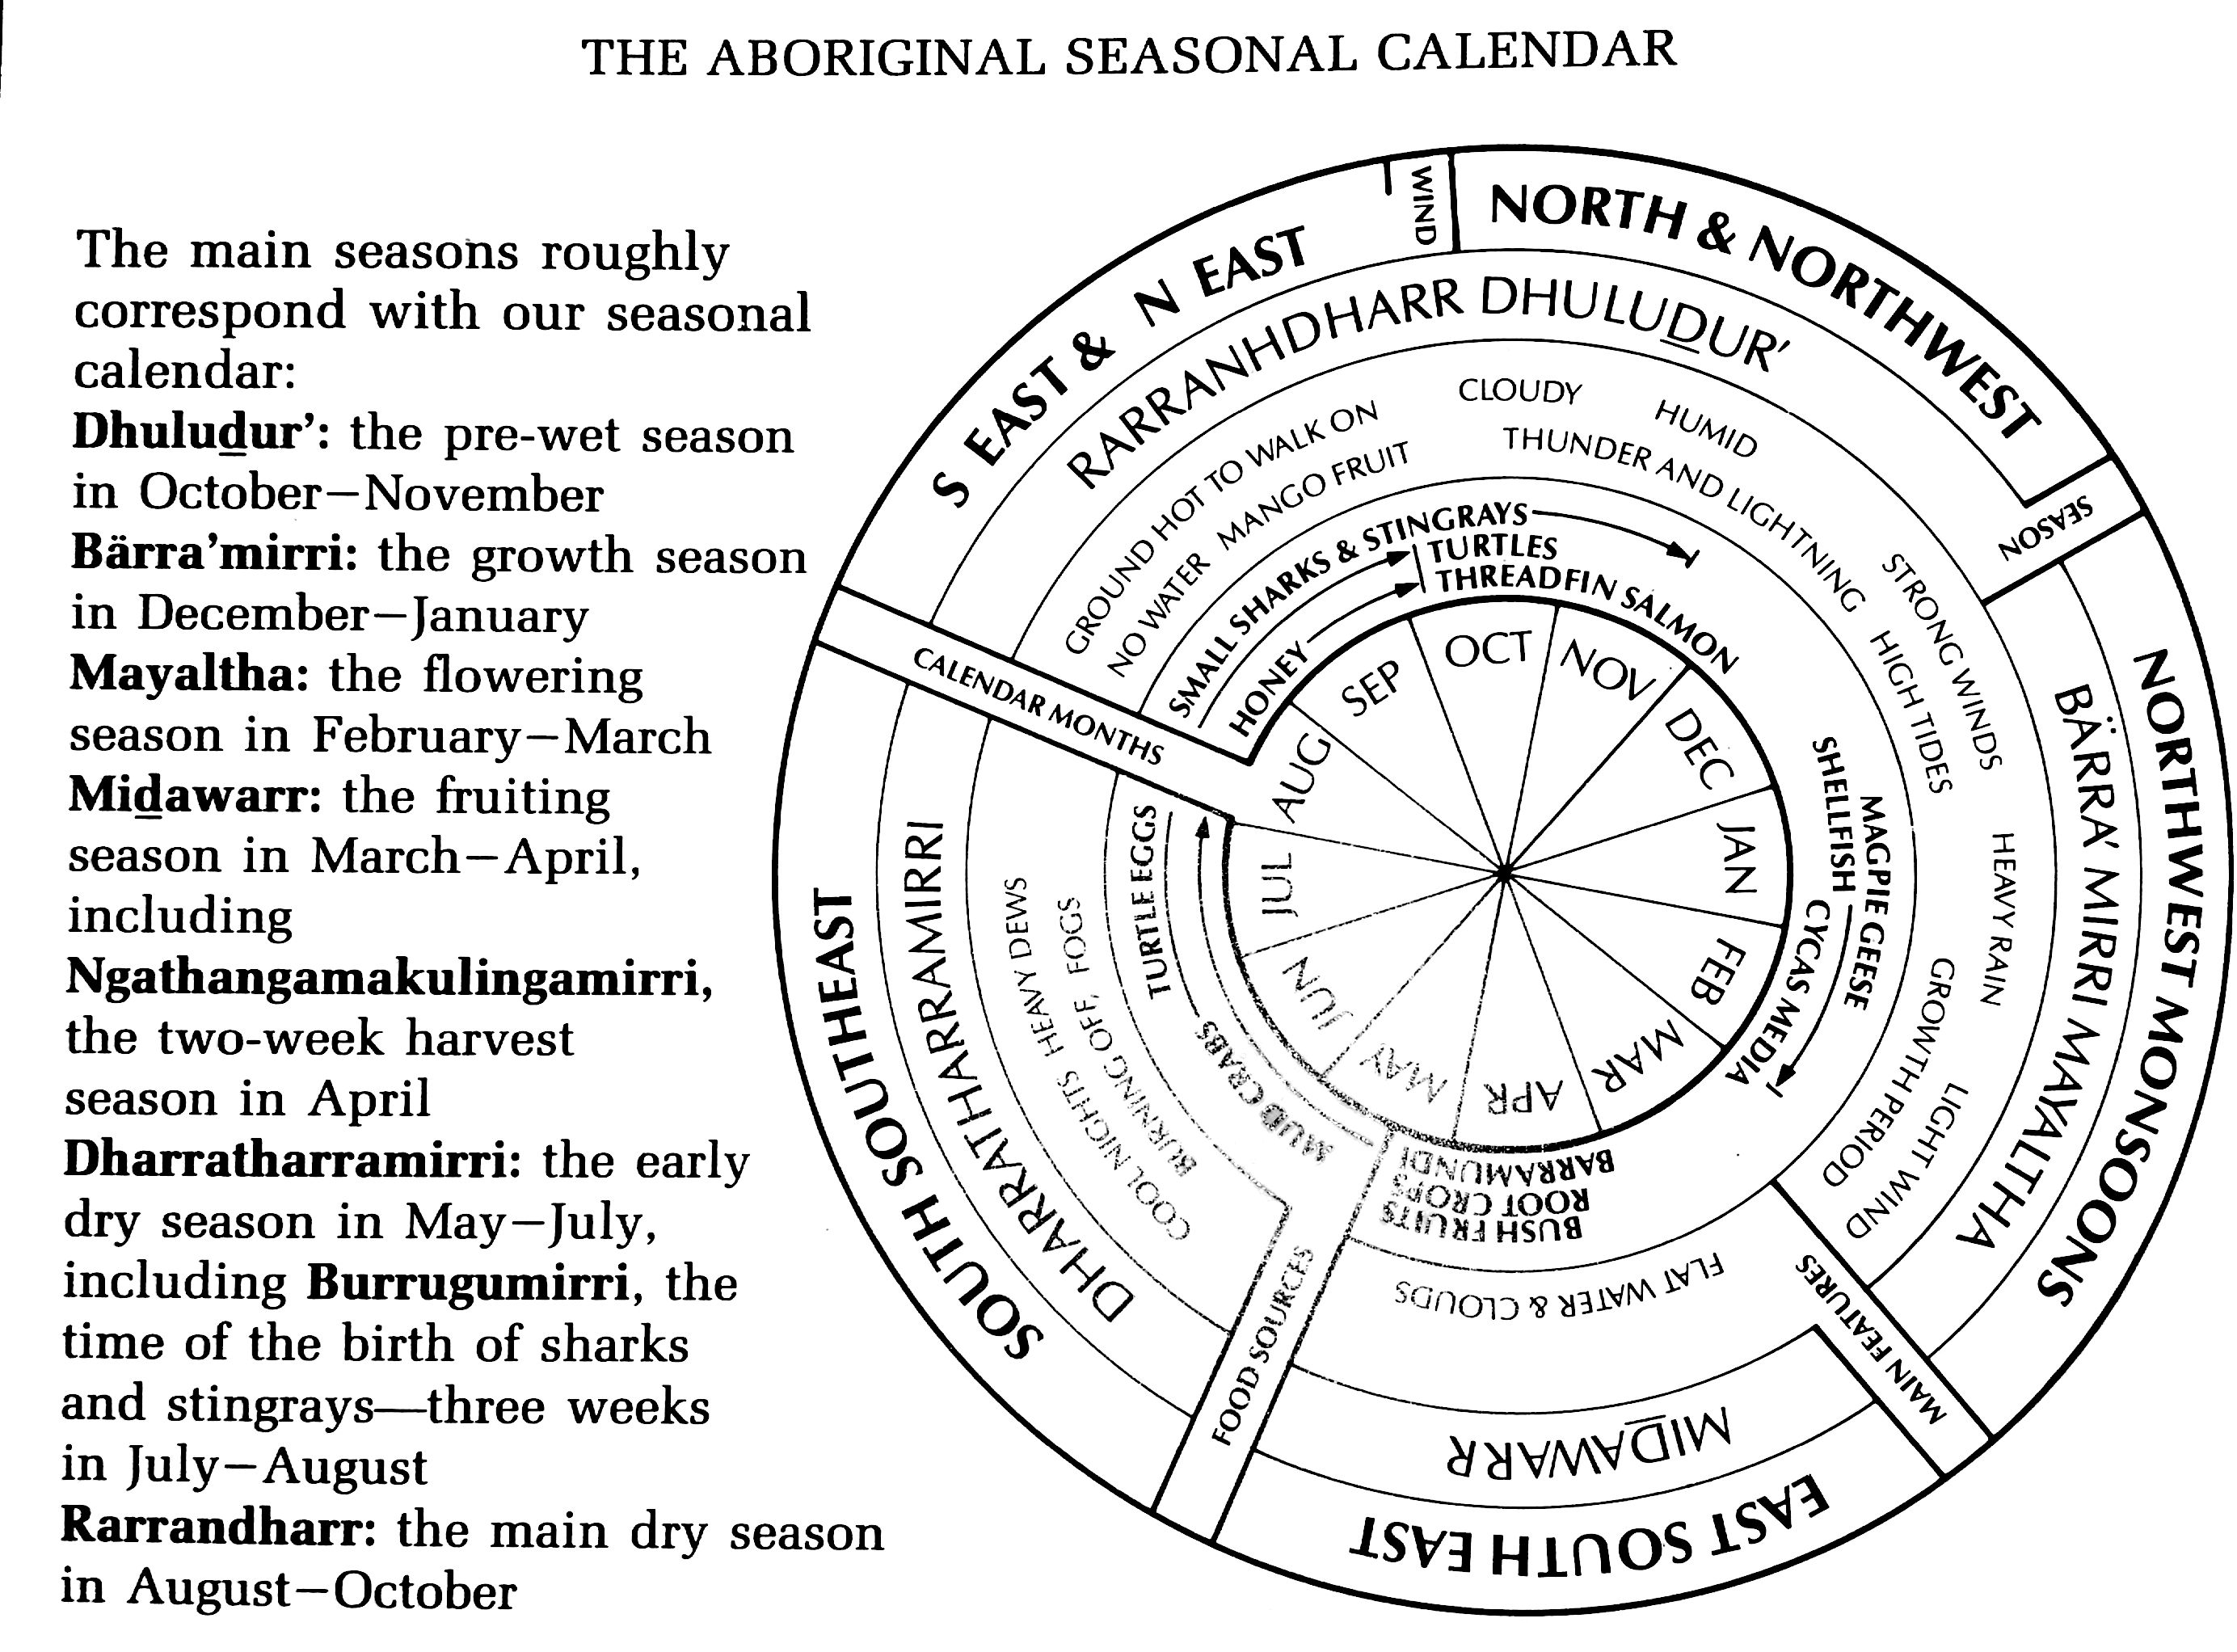
\includegraphics[width=\textwidth]{yolngu-calendar.jpg}
    \caption{Conceptual Yolngu seasonal calendar \citep{davis1989}}
    \label{fig:yolngu-seasons}
\end{figure}


\subsection{Reflection - Complex Calendars as an emergent theme}

`Calendar' and `season' are not concepts that translate directly across cultures. 

Discuss how I realised this, by re-listening to recordings, and that I was
expecting something unforeseen (but not like this!).

Note that informal, collaborative and participant-led conversations were key.

\emph{TODO: expand points to paragraphs, with quotes}

\begin{itemize}
\item all in english
\item what is a season
\item what is a calendar
\item there is no ``the'' yolngu calendar - varies spatially,
        multiple seasonal calendars for different temporal scales with varied purposes
\item `simple fact-finding' really isn't!
\item unusual or extreme events people remember, and how these fit into the calendar
\item understandings of climate change including expected impacts (minimal, after \citet{petheram2010})
\end{itemize}



\subsection{Yolngu Seasons vary by location and temporal scale}

Yolngu participants discussed three levels of seasons:
\begin{itemize}
\item A Wet-Dry seasonality, based on the monsoon winds;
\item A six-season calendar defined primarily by wind, rain, and temperature; and
\item Phenological seasons, where ecological events signal appropriate activities.
\end{itemize}

A similar system is visible in \autoref{fig:tiwi-seasons}, showing the Tiwi seaons at
a monsoonal level, as well as more precise seasons defined by weather or ecology.


\begin{landscape}
\begin{figure}[p]
    \centering
    \includegraphics[width=\paperwidth]{TiwiSeasons.pdf}
    \caption[The Tiwi Seasons Calendar \citep{CSIROcals}]{
        The Tiwi Seasons Calendar \citep{CSIROcals}.
        This calendar shows month of year in the outermost ring,
        then three `major' Tiwi seasons recognised by weather.
        Note that \textit{Kumunupunari} does not have a sharp boundary with \textit{Tiyari}!
        Within this ring are smaller seasons, recognised by weather
        or ecological events and associated with particular activities.
        This format is designed for the circle to rotate, encouraging interaction or observation.
        }
    \label{fig:tiwi-seasons}
\end{figure}
\end{landscape}


\paragraph{Monsoon Seasons (Wet/Dry)}

Of the three levels of seasons recognised by Yolngu,
the wet/dry monsoon seasonal cycle is most likely familiar to non-indigenous people -
especially in the tropics.  Yolngu participants emphasised that these seasons
are \emph{not} recognised by rainfall, but rather the direction of prevailing winds.

\blockquote{
    ADD QUOTE HERE
}

Interestingly, this mirrors the meteorological definition of monsoon,
where rainfall is less important than the location of the intertropical
convergence zone and consequent direction of prevailing wind.
This shared understanding of monsoon seasonality should not go unremarked -
but does direct this research to the more local seasonal patterns.


\paragraph{Meteorological Seasons}

Lorem Ipsum six seasons, using because, details in next subsection.  ADD DETAILS





\paragraph{Phenological Seasons}
Phenological seasons are defined by observed changes in local vegetation
and animal behaviour.  They embody a depth and detail of indigenous
ecological knowledge that is difficult to imagine, and only possible
due to the long connection between Yolngu and the natural environment.

Participants explained that these seasons vary between groups even within
a single clan-nation or language group, meaning that each of the towns
across Arnhem Land (see \autoref{fig:arnhem-map}) would have a different
calendar.  
%
These seasons are closely tied to traditional activities such as travel,
use of particular foods or other resources, and ceremony.

On the Tiwi Seasons Calendar, \autoref{fig:tiwi-seasons}, the inner-most
rings concern phenological seasons and observations - such as
\textit{Mumpikari}, when possums leave muddy tracks and hunting them is easy.

However, certain practicalities put phenological seasons beyond scope
for the remainder of this thesis.
%
The same detail and diversity which makes these seasons so fascinating
also mandates far greater investment of time and travel to speak
with the relevant knowledge holders, and proper study would require
living in each community for a significant period.
%
Sensitive, sacred, or unpublishable stories and information are much more
common around phenological seasons than the more general calendar,
and researchers have obligations in this area which are not always clear.
%
Generalisation between communities is difficult if not impossible.
%
And finally, quantification would be very difficult due to the paucity
of quantitative phenological data at the required level of detail
and localisation, especially in `remote' Australia.




\subsection{Describing a Yolnu Seasonal Calendar}

The remainder of this thesis focusses on a particular Yolnu calendar,
that of six seasons as recognised at Galiwinku on Elcho Island.
See \autoref{fig:yolngu-seasons} for a graphical representation of these seasons.

The descriptions below are drawn from interviews with participants from Galiwinku.
I also present selected quotations from \textit{Man of All Seasons} \citep{davis1989},
which describe the seasons as experienced at Milingimbi.
Note that weather data for both is analysed in \autoref{ch:quantify},
including observations on differences in seasonality.


\paragraph{Dhuludur} marks the beginning of the seasonal cycle.

One participant read \autoref{fig:yolngu-seasons} as claiming Rarrandharr was the first season
and issued a correction, saying \blockquote{XXXXX (find: this before RR.)}.

\citet{davis1989} calls Dhuludur the `pre-wet' season:
\blockquote{
    The weather is cool and still during the night, with mists settling in the night and rising in the morning after a light northwest wind during the day. ...
    The winds are mixed up, with southwest, southeast, northeast, and northwest winds each blowing at different times, often during the same day. ...
    The weather begins to get hot and humid as the clouds build up more and more each day.
    When the sky is covered by heavy cloud, the `female' thunder brings the first rain [often from the southeast].
    After the first rain, other winds bring heavy rain. ...
    
    Towards the end of the pre-wet season the rain is being brought only by the northwest wind.
    It rains almost every evening.
    This is the start of the next season, which is signified by heavy rains and growth.
}

The sea is calm and the skies are clear.


\paragraph{Barramirri}

\citet{davis1989} calls Barramirri `the season of heavy rain and growth':
\blockquote{
    The heavy rain is brought by the northwest wind. It comes every day, indicating that the seasons have changed. ...
    As the northwest wind brings daily storms, the sea is dirty and rough. ...
    The inundation is so extensive that much of the inland is now one continious sheet of water [, which will not drain until the end of the wet season]. ...
    
    Many plants flower, an the rain becomes infrequent and sometimes stops for several weeks.
    These are indications that the season of heavy rain is drawing to a close.
}


\paragraph{Mayaltha} is the season of plenty - at Galiwinku.  

QUOTE R on whatever tye of food, how to recognise season.

\citet{davis1989} calls Mayaltha the `flowering' season:
\blockquote{
    [The Flowering Season] is marked by an abundance of plants that flower, bright sunny days, cool breezes, and occasional rain. ...
    
    During the early wet season strong winds often brought the rain.
    The wind then stopped as the rain fell.
    Now the winds blow hard even when it is raining.
    The rains do not come daily any more, but only every week or two.
}


\paragraph{Midawarr} is recognised at Milingimbi as the season of plenty, but folded into Mayaltha at Galiwinku.

Some participants did not name this as a separate season.
It is instead seen as part of Mayaltha, which becomes a major season - along with wet and dry.
This is a concrete example of the variation in calendars between communities and the complexity of seasons over different timescales,
making them a rich source of ecological knowledge and a frustrating subject of study!

\citet{davis1989} calls Midawarr the `fruiting' season:
\blockquote{
    The east wind signals the beginning of the time of abundant food ... the first southeast wind blows gently in the early morning. ...
    
    The daily storms and strong winds are nearly over.  The northwest wind changes to the northeast, bring rough seas.
    Early in the season the storms still bring heavy rain daily.
    
    By the middle of the season the wind has changed to the east and heavy storms are less frequent.
    Light easterly winds blow throughout most of the day bringing cooler weather. ...
    
    Shortly after sunrise the east wind blows and continues for the rest of the day.
    
    Towards the end of the fruiting season, the days are becoming more like the early dry season with morning mists.
    One last storm of the wet season comes and flattens the tall dry grass.
    This storm is brought by strong southeast wind, which is the main dry season wind.
}


\paragraph{Dharrathamirri}

\citet{davis1989} calls Dharrathamirri the `early dry' season:
\blockquote{
    In the early dry season the night sky is again mostly clear and the three stars of
    \textit{Djulpan} (Orion's Belt) are seen in the west in the early night sky,
    and reach the horizon before people go to sleep.
    This is the time when the storms come and knock the grass down.
    
    When the rain has stopped and the southeast wind is blowing constantly, the dry season has really started.
    
    After the first storm the wind varies in direction.
    Heavy dews come with the light ESE to SE wind that blows every night.
    When we are well into the season the wind swings SE to SSE and becomes stronger
    
    The southeast wind blows stronger in the latter half of the season.
    
    The next season does not start immediately.
    The northeast, southwest, and southeast winds vary for a few weeks.
}


\paragraph{Rarrandharr}

\citet{davis1989} calls Rarrandharr the `main dry' season:
\blockquote{
    The east-southeast wind blows; the cold mornings and mist are nearly gone.
    This is an intermediate season between the early dry and main dry seasons.
    It is very short, lasting only a few weeks.
    
    The warmer southeast wind starts to blow...
    When the wind dies down, soon the three stars of \textit{Djulpan} will begin to rise in the east before people go to sleep at night.
    
    When the mangoes are nearly finished, the dry season is also near its end.
    The weather changes and thunder begins.
}








